% vim:autoindent:set textwidth=78:

\section{Compositore di stampe}\label{label_printcomposer}

% when the revision of a section has been finalized, 
% comment out the following line:
% \updatedisclaimer

Il compositore di stampe fornisce funzionalità per la creazione di layout di
stampa che saranno continuamente migliorate. Consente di aggiungere elementi
al layout come la vista mappa, la legenda, la barra di scala, immagini esterne
e campi testuali. È possibile cambiare le dimensioni, raggruppare e spostare
ogni elemento e regolarne le proprietà per creare il layout desiderato. 
Il risultato può essere stampato (anche come Postscript e PDF), esportato come
immagine o come disegno vettoriale in formato SVG.\footnote{L'esportazione in
SVG è supportata, ma non funziona correttamente con alcune recenti versioni di
QT4. È necessario fare delle prove e dei controlli individuali sul proprio
sistema} Si veda l'elenco degli strumenti nella tabella~\ref{tab:printcomposer_tools}:

\begin{table}[h]\index{Print composer!tools}
\centering
\caption{Strumenti del compositore di stampe}\label{tab:printcomposer_tools}\medskip
 \begin{tabular}{|l|p{6.9cm}|l|p{6.9cm}|}
 \hline \textbf{Icona} & \textbf{Scopo} & \textbf{Icona} &
 \textbf{Scopo} \\

 \hline 
\includegraphics[width=0.7cm]{mActionExportMapServer}
 & Esporta come immagine & 
 
\includegraphics[width=0.7cm]{mActionSaveAsSVG} & Esporta come SVG \\
 \hline 
\includegraphics[width=0.7cm]{mActionFilePrint} & Stampa o esporta
 come PDF o Postscript &
 
\includegraphics[width=0.7cm]{mActionZoomFullExtent} & Zoomma all'estensione
 massima \\
 \hline 
\includegraphics[width=0.7cm]{mActionZoomIn} & Ingrandisci &
 
\includegraphics[width=0.7cm]{mActionZoomOut} & Rimpicciolisci \\
 \hline 
\includegraphics[width=0.7cm]{mActionDraw} & Aggiorna la vista &
 
\includegraphics[width=0.7cm]{mActionAddRasterLayer} & Aggiungi una nuova
 vista mappa da QGIS \\
 \hline 
\includegraphics[width=0.7cm]{mActionSaveMapAsImage} & Aggiungi
 immagine al layout di stampa &
 
\includegraphics[width=0.7cm]{mActionLabel} & Aggiungi caselle di testo al
 layout di stampa \\
 \hline 
\includegraphics[width=0.7cm]{mActionAddLegend} & Aggiungi una nuova
 legenda al layout di stampa & 
 
\includegraphics[width=0.7cm]{mActionScaleBar} & Aggiungi una barra di scala
 al layout di stampa\\
 \hline 
\includegraphics[width=0.7cm]{mActionSelectPan} & Seleziona/sposta
 oggetti del layout di stampa &
 
\includegraphics[width=0.7cm]{mActionMoveItemContent} & Sposta centro della
 vista mappa \\
 \hline 
\includegraphics[width=0.7cm]{mActionGroupItems} & Raggruppa oggetti
 del layout & 
 
\includegraphics[width=0.7cm]{mActionUngroupItems} & Separa oggetti del
 layout \\
 \hline 
\includegraphics[width=0.7cm]{mActionRaiseItems} & Alza di livello
 l'oggetto selezionato nel layout &
 
\includegraphics[width=0.7cm]{mActionLowerItems} & Abbassa di livello
 l'oggetto selezionato nel layout \\
 \hline 
\includegraphics[width=0.7cm]{mActionMoveItemsToTop} & Porta l'oggetto
 selezionato in primo piano & 
 
\includegraphics[width=0.7cm]{mActionMoveItemsToBottom} & Porta l'oggetto
 selezionato sullo sfondo \\
\hline
\end{tabular}
\end{table}

Per accedere al compositore di stampe, cliccare sul pulsante
\toolbtntwo{mActionFilePrint}{Print} nella barra strumenti o scegliere la voce
di menù \mainmenuopt{File} > \dropmenuopttwo{mActionFilePrint}{Compositore
stampe}.

\subsection{Uso del compositore di stampe}\label{label_useprintcomposer} 

Prima di iniziare a lavorare con il compositore di stampe, è necessario
caricare alcuni livelli raster e vettoriali nella vista mappa di QGIS e
regolarne le proprietà secondo le proprie esigenze. Una volta effettuate
tutte le impostazioni e applicata la simbologia cliccare sul pulsante
\toolbtntwo{mActionFilePrint}{Compositore stampe}.

\begin{figure}[ht]
   \begin{center}
   \caption{Compositore di stampe \nixcaption}\label{fig:print_composer_blank}\smallskip
   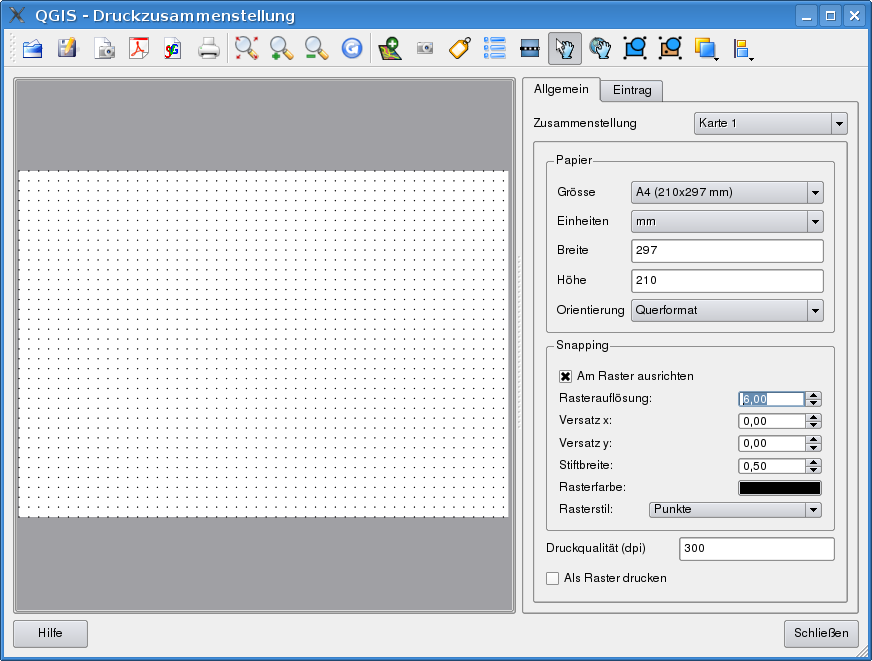
\includegraphics[clip=true, width=\textwidth]{print_composer_blank}
\end{center}  
\end{figure}

Aprendo il compositore di stampe viene visualizzato un foglio bianco al quale
aggiungere vista mappa, legenda, barra di scala, immagini e testo. La Figura
\ref{fig:print_composer_blank} mostra la vista iniziale del compositore di
stampe prima dell'aggiunta di un qualunque elemento. Nel compositore di stampe
co sono due linguette:

\begin{itemize}
\item La linguetta \tab{Generale} consente di impostare la dimensione del
foglio, l'orientamento e la qualità di stampa del file in uscita in dpi.
\item La linguetta \tab{Oggetto} mostra le proprietà dell'elemento selezionato
nel layout di stampa. 
Cliccare sull'icona \toolbtntwo{mActionSelectPan}{Seleziona/Sposta oggetto} 
per selezionare un elemento (ad es. legenda, barra di scala o etichetta
testuale) nel layout. Cliccare dunque sulla linguetta \tab{Oggetto} e
personalizzare le impostazioni dell'elemento selezionato.
\end{itemize}

Possono essere aggiunti diversi elementi al compositore ed è anche
possibile avere più di una vista mappa o legenda o barra di scala nel layout
di stampa. Ogni elemento ha le sue proprietà e, nel caso delle viste mappa, la
propria estensione.

\subsubsection{Aggiungere una vista mappa al layout nel compositore di
stampe}

Per aggiungere una vista mappa, cliccare sul pulsante
\toolbtntwo{mActionAddRasterLayer}{Aggiungi nuova mappa} nella barra strumenti
del compositore di stampe e trascinare il mouse per definire un rettangolo
nell'area occupata dal foglio tenendo premuto il tasto sinistro per aggiungere
la vista mappa. Verrà visualizzato un riquadro vuoto con la scritta
\textit{"La mappa verrà stampata qui"}. Per visualizzare effettivamente la mappa,
selezionare \selectstring{Anteprima}{Cache} nella linguetta \tab{Oggetto}.

\begin{figure}[ht]
\centering
\caption{Contenuti della linguetta Oggetto nel compositore di stampe \nixcaption}\label{fig:print_composer_map_item}
   \subfigure[Sezione per definizione larghezza, altezza ed estensione] {\label{subfig:print_composer_map_item1}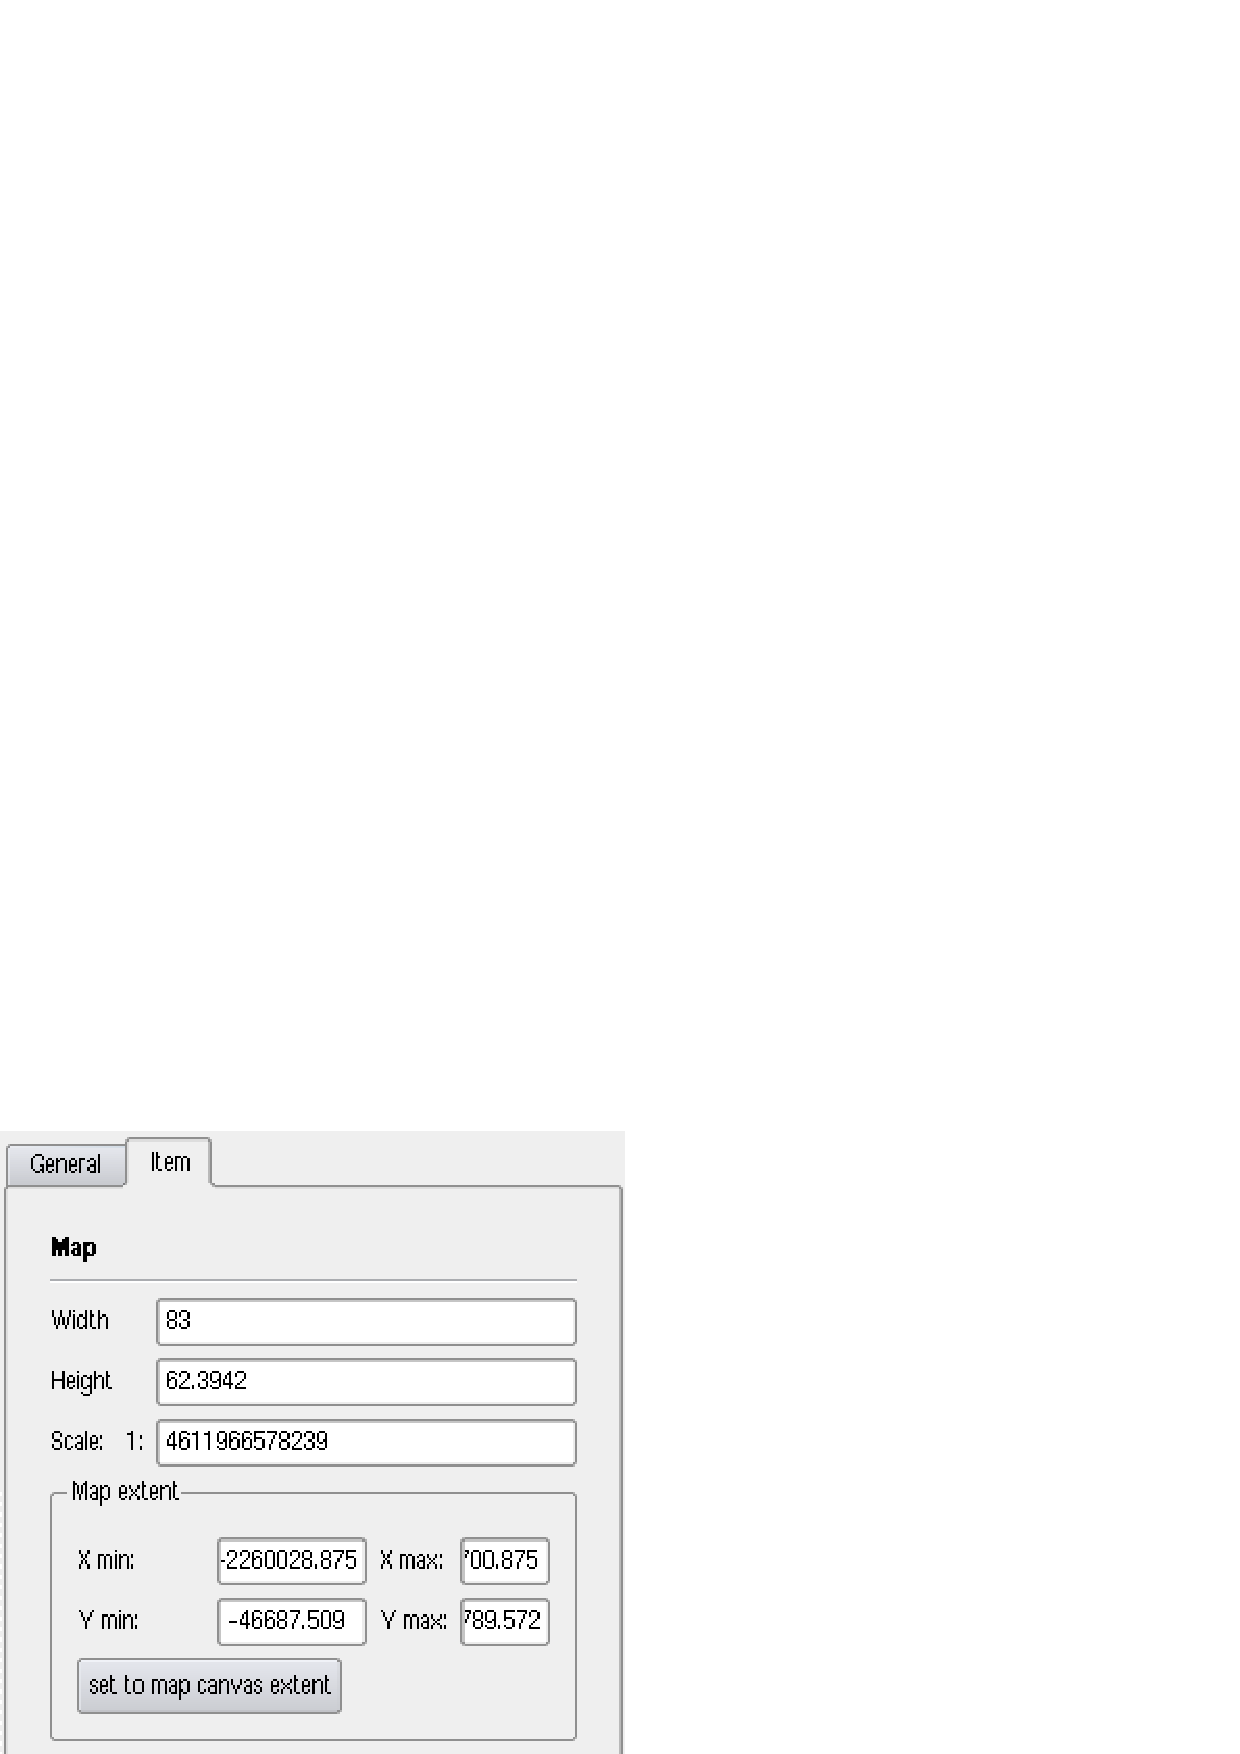
\includegraphics[clip=true, width=0.4\textwidth]{print_composer_map_item1}}\goodgap
   \subfigure[Sezione proprietà] {\label{subfig:print_composer_map_item2}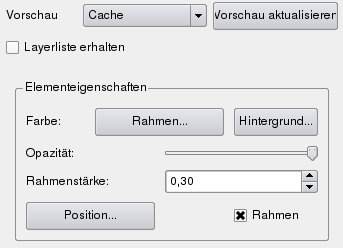
\includegraphics[clip=true, width=0.4\textwidth]{print_composer_map_item2}}
\end{figure}

È possibile ridimensionare la mappa in un momento successivo cliccando sul
pulsante \toolbtntwo{mActionSelectPan}{Seleziona/Sposta oggetto}, selezionando
un elemento e trascinando una delle maniglie blu agli angoli della mappa. Con
la mappa selezionata, è possibile regolare ulteriori proprietà della vista
mappa nella linguetta \tab{Oggetto}. Ridimensionare la mappa specificando la
larghezza e l'altezza o la scala. Definire l'estensione della mappa usando i
valori massimi/minimi per gli assi X e Y o cliccando sul pulsante
\button{Imposta all'estensione della mappa}. Aggiornare l'anteprima della
mappa e selezionare se si desidera avere un'anteprima della mappa dalla cache
o un rettangolo vuoto con il messaggio \textit{"La mappa verrà stampata qui"}.
Definire i colori e lo spessore del contorno della cornice dell'elemento,
impostare un colore di sfondo e l'opacità del foglio mappa. È anche possibile
scegliere se visualizzare o meno una cornice attorno agli elementi con la
casella di controllo \checkbox{Cornice} (si veda la
Figura~\ref{fig:print_composer_map_item}). Se si modifica la vista mappa nel
programma zoommando o spostando la vista o cambiando le proprietà dei
vettoriali o dei raster, è possibiel aggiornare la vista nel compositore di
stampe cliccando sul pulsante \button{Aggiorna la vista} nella linguetta
\tab{Oggetto} (si veda la Figura~\ref{fig:print_composer_map_item}). 

Per spostare l'area visualizzata nella vista mappa aggiunta nel compositore,
cliccare sul pulsante \toolbtntwo{mActionMoveItemContent}{Sposta contenuto
oggetto} e spostare la vista nella cornice della vista mappa trascinando con
il tasto sinistro del mouse premuto.

\begin{Tip}\caption{\textsc{Salvare un layout di stampa}}
\qgistip{Se si desidera salvare lo stato attuale di una sessione del
compositore di stampe, cliccare su \mainmenuopt{File} >
\dropmenuopttwo{mActionFileSaveAs}{Salva Progetto con nome} per salvare lo
stato dello spazio di lavoro incluso quello della sessione attuale del
compositore di stampe. In futuro sarà possibile salvare separatamente lo stato
del compositore di stampa.
}
\end{Tip} 

\subsubsection{Aggiunta di altri elementi al compositore di stampa} 

Oltre ad aggiungere una vista mappa al layout di stampa, è anche possibile
aggiungere, spostare e personalizzare legenda, barra di scala, immagini e
caselle testuali.

\minisec{Etichette ed immagini}

Per aggiungere una etichetta o un'immagine, cliccare sugli strumenti
\toolbtntwo{mActionLabel}{Aggiungi nuova etichetta} o
\toolbtntwo{mActionSaveMapAsImage}{Aggiungi immagine} e posizionare gli
elementi con il tasto sinistro del mouse al layout di stampa.

\begin{figure}[ht]
\centering
\caption{Personalizzazione di immagini ed etichette nel layout di stampa \nixcaption}\label{fig:print_composer_tab2}
   \subfigure[Linguetta oggetto per le etichette] {\label{subfig:print_composer_label_item}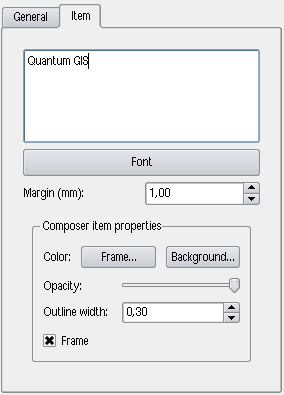
\includegraphics[clip=true, width=0.4\textwidth]{print_composer_label_item}}\goodgap
   \subfigure[Linguetta oggette per l'immagine] {\label{subfig:print_composer_image_item}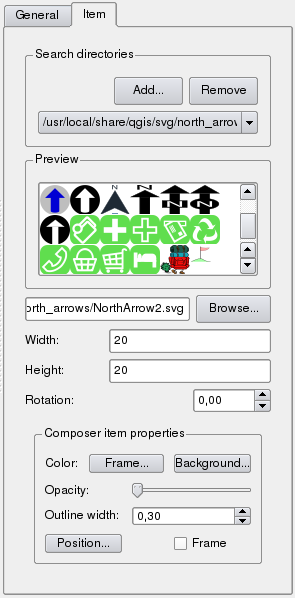
\includegraphics[clip=true, width=0.4\textwidth]{print_composer_image_item}}
\end{figure}

\minisec{Legenda e barra di scala}

Per aggiungere una legenda o una barra di scala, cliccare sul pulsante
\toolbtntwo{mActionAddLegend}{Aggiungi nuova legenda vettoriale} o
\toolbtntwo{mActionScaleBar}{Aggiungi nuova barra di scala} e posizionare
l'elemento con il tasto sinistro del mouse nel layout di stampa.

\begin{figure}[ht]
\centering
\caption{Personalizzazione della legenda e della barra di scala nel
compositore di stampe \nixcaption}\label{fig:print_composer_tab1}
   \subfigure[Linguetta oggetto per la legenda] {\label{subfig:print_composer_legend_item}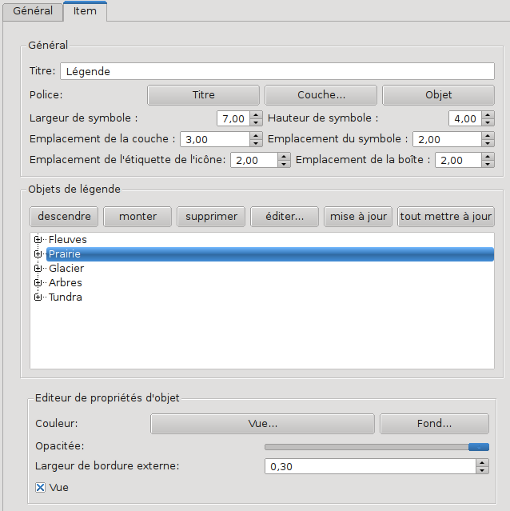
\includegraphics[clip=true, width=0.4\textwidth]{print_composer_legend_item}}\goodgap
   \subfigure[Linguetta oggetto per la barra di scala] {\label{subfig:print_composer_scalebar_item}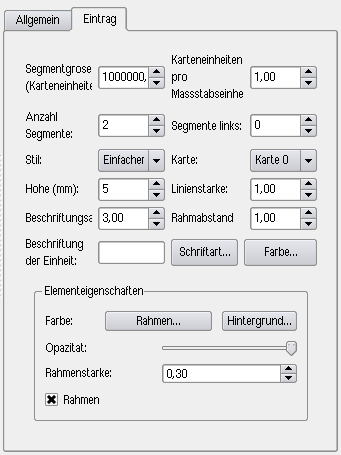
\includegraphics[clip=true, width=0.4\textwidth]{print_composer_scalebar_item}}
\end{figure}

\subsubsection{Strumenti per l'esplorazione del layout di stampa}

Per l'esplorazione del layout nel compositore di stampe sono forniti 4
strumenti:

\begin{itemize}
\item \toolbtntwo{mActionZoomOut}{Ingrandisci},
\item \toolbtntwo{mActionZoomOut}{Rimpicciolisci},
\item \toolbtntwo{mActionZoomFullExtent}{Vista ad estensione massima} e
\item \toolbtntwo{mActionDraw}{Aggiorna la vista}, che serve nel caso in cui
la vista nel layout non rispecchi quanto presente nella vista mappa in QGIS. 
\end{itemize}

\subsubsection{Creazione di file in uscita}

La Figura \ref{fig:print_composer_complete} mostra il compositore di stampe
con un layout di stampa completo di ognune degli elementi precedentemente
descritti.

\begin{figure}[h]
   \begin{center}
   \caption{Compositore di stampe con layout completo di vista mappa, legenda,
   barra di scala e testo \nixcaption}
   \label{fig:print_composer_complete}\smallskip
   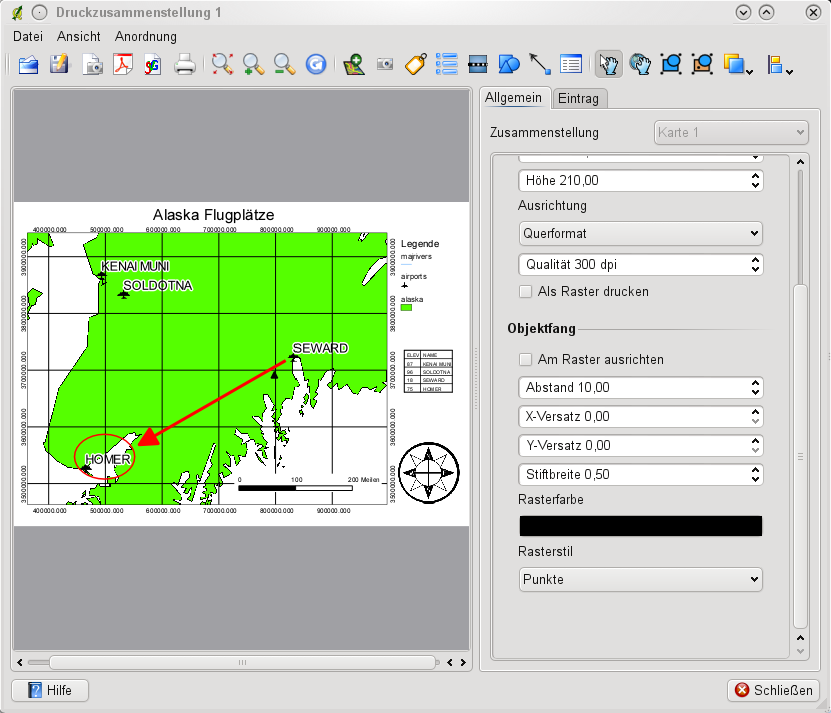
\includegraphics[clip=true, width=\textwidth]{print_composer_complete}
\end{center}  
\end{figure}

Il compositore di stampe consente di creare diversi formati in uscita ed è
possibile definirne la risoluzione (qualità di stampa) e il formato pagina:

\begin{itemize}
\item L'icona \toolbtntwo{mActionFilePrint}{Stampa} consente di stampare il
layout su una stampante collegata o su un file PDF o Postscript in funzione
del driver stampante installato.
\item L'icona \toolbtntwo{mActionExportMapServer}{Esporta come immagine}
esporta il layout in diversi formati immagine come PNG, BPM, TIF, JPG, \dots
\item L'icona \toolbtntwo{mActionSaveAsSVG}{Esporta come SVG} salva il layout
di stampa in formato SVG (Scalable Vector Graphic). \textbf{Nota:} Attualmente
l'uscita in SVG è ad un livello molto iniziale. Il problema non sta in QGIS,
ma nella sottostante libreria Qt. Ci si augura che questo problema venga
risolto nelle prossime versioni della libreria.
\end{itemize}

